%
%   latex writeup for KeystrokeAuth
%   6.858 Final Project
%   December 2013
%   forrestp, ameeshg, kseibert, cbieden
%
%

\documentclass{article}

\usepackage{geometry}
\geometry{letterpaper}

\usepackage{doc}

\usepackage{graphicx}
\usepackage{float}
\usepackage{caption}
\usepackage{subcaption}

\usepackage{epstopdf}

\usepackage{enumitem}
\setdescription{leftmargin=\parindent,labelindent=1cm}

\title{KeystrokeAuth}
\author{
  Forrest Pieper\\
  Kenneth Seibert\\
  Ameesh Goyal\\
  Carlo Biedenharn
}
\date{December 13th, 2013}

\begin{document}

\maketitle

\abstract{
}

\section{Introduction}
\label{introduction}
KeystrokeAuth is an example website implementation that uses keystroke timing to provide stronger user authentication.
Measuring keystroke timing is a method for passive biometric authentication. 
Traditional biometric authentication such as fingerprint or retinal scanners require external hardware and is not suited for web service authentication where users may login from a variety of machines. 
Keystroke timing can be gathered using Javascript embedded in the login and registration pages.
Thus this method requires no additional hardware.
The user must enter her password several times during registration instead of just once or twice, but otherwise the method is largely unobstrusive.
Authenticating passwords with keystroke timing makes it more difficult for an attacker who possesses a user's plaintext password to compromise the account.
Additionally, it discourages account sharing which may be useful for highly secure systems and premium accounts.
In this paper we describe past work on the topic, introduce our example implementation, analyze the added security of our system, and examine a small set of test data.

\section{Background and Related Work}

Many different studies have been done in the past about fingerprinting users based on keystroke cadence, two of which are referenced below. However, many of these studies focus on running a keylogger in the background of a user session and collecting a large amount of keystrokes before making a decision. The training data that these keystrokes are compared to can also be quite large. In contrast, KeystrokeAuth can only compare the timing data from a short password entry to the timing data of a small bank of previously entered passwords. This makes detecting adversaries much more difficult.

In our system, we avoided the legwork of comparing multiple algorithms for what may be the best fit for us. Instead, we chose a few of the top performing algorithms described in {[}1{]} to test in a password context with a much smaller bank of training data (in contrast to 400 in the paper). In particular, the Mahalanobis distance described below performed very well in {[}1{]} and is described in more detail in {[}2{]}. We believe that a bank of 400 passwords is unrealistic for most websites to request of a user. In KeystrokeAuth, we settle on 10 password entries upon registration, which is much more reasonable. 

\section{KeystrokeAuth Implementation}
KeystrokeAuth is a Flask website that uses Javascript to capture the timestamps on each keydown and keyup event while typing the password.
During registration, the user enters her password 10 times.
The data is sent to the server and KeystrokeAuth computes a model specific to that user and password.
When logging in, the user enters the password once and KeystrokeAuth compares the new timing data to the registered training data.
If the timing data differs too much, the user will not be logged in.

\subsection{Gathering Timing Data}
Timing data is gathered with Javascript event handlers on key presses in the registration and login pages.
Timing data is only gathered when the focus is on the password field. The password field is reset whenever it gains focus (via the onFocus event handler).  
While gathering timing data, any key that is not a valid password character, e.g. backspace or the arrow keys, causes the entire password field to reset.
This ensures we only get timing data for a continous entry of password characters.

The timing data for each password entry consists of a list of objects with keycode, keyup, and keydown fields. The keyup and keydown fields are timestamps normalized by subtracting the keydown timestamp for the first character in the password entry. 
During login, only one password entry is gathered. During registration, a counter keeps track of enteries and won't submit until the password has been entered 10 times.

Some tables and logs indicating which of the models passed and failed are printed out to the page after submission of the login page. 
This is useful for debugging purposes, but should be turned off for a real-world implementation.

\subsection{Generating User Timing Models}
In order to have success with verifying users using keystroke dynamics, we first have to establish the set of training data. The keystroke dynamics that we are interested in include the following:
\begin{description}
	\item[Down time:] The time that each key is pressed down at, where the first key pressed down equates to a time of zero
	\item[Down-Down time:] The time in-between two consecutive key down events
	\item[Flight time:] The time in-between a key up and the following key down event. This value can be negative as a key may not be released before the next is pressed down. 
	\item[Dwell time:] The time that a given key is held down
\end{description}
We are able to calculate all of these values from the initial 10 password entries that are passed in during registration. These metrics will be passed to the distance algorithm described below to deterimine if the entry is close enough to permit login.

\subsection{Login Authentication Algorithm}
We make use of the Mahalanobis distance to compute the similarity between two password timings, represented as vectors.  \\
\begin{displaymath}
D_m(\vec{x}) = \sqrt{(\vec{x}-\vec{y})^T S^{-1} (\vec{x}-\vec{y})}
\end{displaymath} \\
Mahalanobis distance is used in two different authentication functions. The first function takes the mean of the training data vectors and computes the distance between the login attempt and the computed mean vector. If the distance from the mean vector is below a certain threshold the login attempt is accepted. 

The 2nd function that we employ takes the login attempt and finds its distance from each of the training vectors. If the $k$ closes distances all fall below a threshold the login attempt is accepted.
 
The threshold is computed using the training data. We find the Mahalanobis distance between each vector in the training data ($n^2$ distances). We then compute the average distance. The threshold is set to be one standard deviation away from the mean in the direction of smaller distances. In other words we only accept login attempts where the distance of the attempt is within one deviation from our computed mean distance. We found that this worked better than a universal threshold because some users are more erratic in their password entry.

\section{Security Analysis}
KeystrokeAuth makes it more difficult for an attacker with knowledge of a user's plaintext password to gain access to the user's account.
Users should still try to keep their passwords secret.
Since KeystrokeAuth is intended to augment standard password-based authentication for web services, it must not weaken any of the security featurus of the standard scheme. 
For it to be useful in practice, the login process must not be much more difficult for actual users.
At the same time, the login process should be more difficult for an attacker with a user's plaintext password.

The following two terms are useful for describing how KeystrokeAuth meets these goals:

\begin{description}
  \item[False Negative:] When an authentic user enters the correct password but is not logged in. If the false negative rate is high, users will get very annoyed about not being able to log in consistently.
  \item[False Positive:] When an attacker enters the correct password and is logged in. If the false positive rate is 100\%, the security is the same as standard password authentication.
\end{description}

The threshold described in 3.3 can be adjusted to affect the error rates. 
Making the threshold smaller increases the false negative rate but decreases the false positive rate, and vice versa.
In our authentication algorithm, the threshold is set such that the false negative rate is around 30\%. Although this seems high, 90\% of users will login within 2 tries. This is a good tradeoff between security and convenience because our false positive rate is significanlty less than 100\%.

The standard password security strategy allows for the password database to be compromised without revealing the users password.
KeystrokeAuth was carefully designed not to violate this security feature.

The timing model for each user is encrypted with AES CFB encryption using a salted and hashed (PBKDF2) user password as the key. The salt in this case differs from the salt and hash of the user password that is stored on the server. Thus, for each user, the server stores the username, two different salts, the hashed and salted password, and the encrypted timing data. 
An attacker with a compromised copy of the database but no plaintext password would not be able to unencrypt this model, preventing him from using the timing information to guess the password.
An attacker with the plaintext password but no copy of the database would have no way of determining the user's timing model, so his only option would be to try to log in many times with various typing rhythms. 

An attacker with both the plaintext password and a copy of the database would be able to decrypt the model and use a script to send keypresses at the correct times to compromise the account. 
Of course, in standard password authentication the attacker wouldn't even need the copy of the database. KeystrokeAuth is more secure in this regard.



\section{Data Collection and Analysis}

\subsection{Data Overview}
Timing data was recorded from twelve participants typing three phrases. In an effort to record relevant data while not divulging the passwords of the participants, familiar phrases were used. Each participant was instructed to type each phrase at least ten times, in any order. Each participant had to type the same three phrases: \textit{facebookgoogle}, \textit{phideltatheta}, and \textit{biedenharn}.\\

The phrase \textit{facebookgoogle} was chosen as it is universally familiar to our participants, resulting in very consistent typing rhythms. \textit{phideltatheta} was used because a portion of our participants were familiar with the phrase. The last phrase, \textit{biedenharn}, was chosen as an example of an attack where \textit{biedenharn} was the account password of a user and the participants were trying to compromise the account. Like a password, \textit{biedenharn} was not familiar to any of our participants except for one of the authors of this paper.\\

Even when looking at the messy graph in Figure \ref{full_facebookgoogle_flight}, it is clear that individuals have unique typing rhythms with familar words. Filtering the data down to a few participants in Figure \ref{multi_facebookgoogle_flight} shows this more directly.

\begin{figure}[H]
  \begin{subfigure}[b]{75mm}
    \centering
    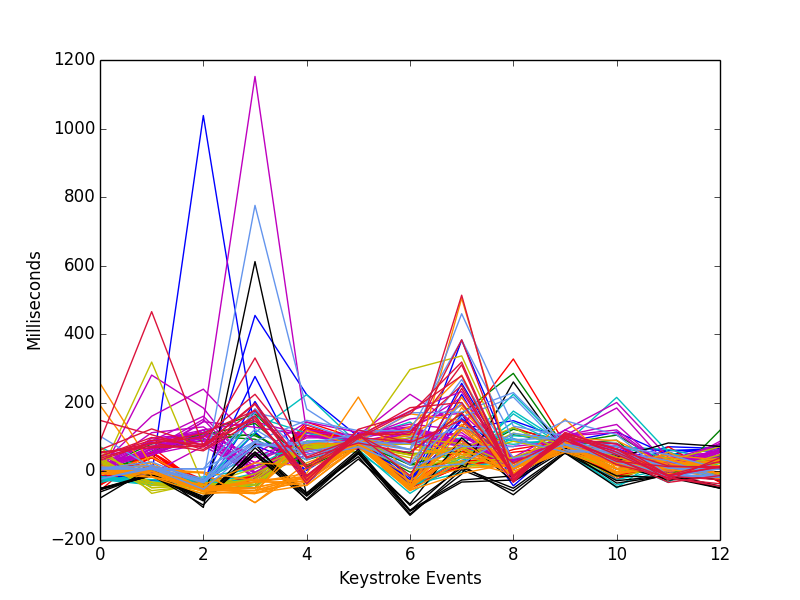
\includegraphics[width=70mm]{facebookgoogle_flight_final.png}
    \caption{All data}
    \label{full_facebookgoogle_flight}
  \end{subfigure}
  \begin{subfigure}[b]{75mm}
    \centering
    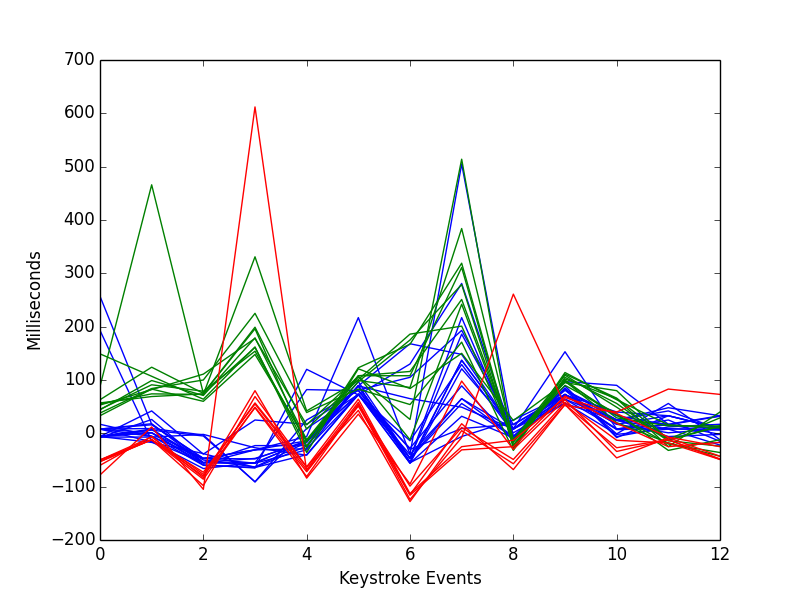
\includegraphics[width=70mm]{facebookgoogle_multi_flight_final.png}
    \caption{Three individuals}
    \label{multi_facebookgoogle_flight}
  \end{subfigure}
  \caption{Flight measurements for participants typing \textit{facebookgoogle}. Each distinct color represents an individual.}
\end{figure}

\subsection{Feature Comparison} 

In practice, the different features produce variably unique datasets. Though the graphs comparing the \textit{up} and \textit{down} features are unique, it is easy to see in figure \ref{all_graphs:down} that with practice an attacker might be able to replicate a victim's data. However with the \textit{flight} and \textit{down-down} graphs (figures \ref{all_graphs:flight} and \ref{all_graphs:down-down}), the results are very consistent and unique. The green dataset has mostly positive flight times while the blue dataset has mainly negative times.

\begin{figure}[H]
  \centering
  \begin{subfigure}[b]{0.3\textwidth}
    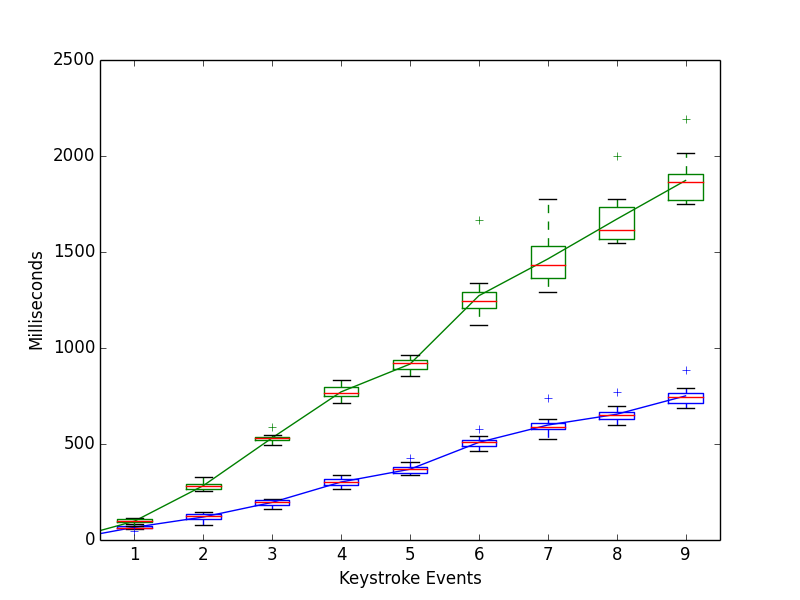
\includegraphics[width=\textwidth]{biedenharn_jordan_down_final.png}
    \caption{down}
    \label{all_graphs:down}
  \end{subfigure}%
  ~ %add desired spacing between images, e. g. ~, \quad, \qquad etc.
    %(or a blank line to force the subfigure onto a new line)
  \begin{subfigure}[b]{0.3\textwidth}
    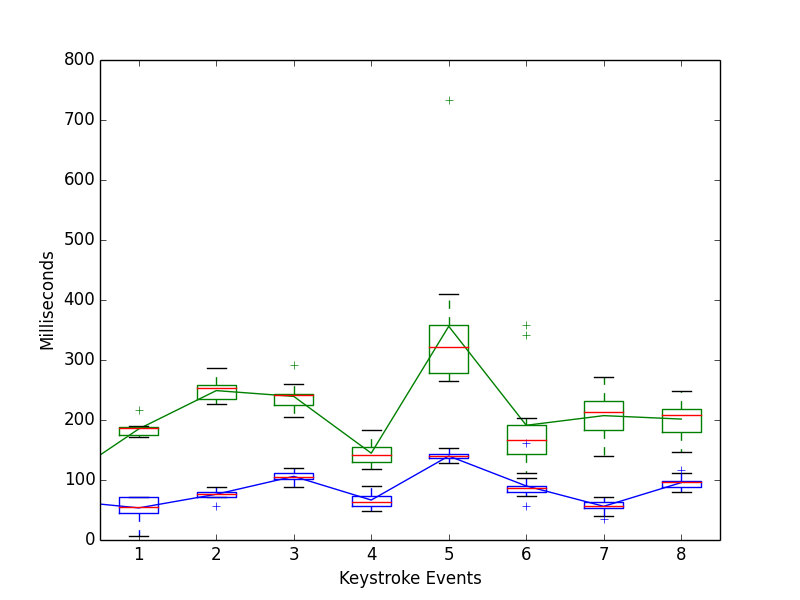
\includegraphics[width=\textwidth]{biedenharn_jordan_down-down_final.png}
    \caption{down-down}
    \label{all_graphs:down-down}
  \end{subfigure}
  ~ %add desired spacing between images, e. g. ~, \quad, \qquad etc.
    %(or a blank line to force the subfigure onto a new line)
  \begin{subfigure}[b]{0.3\textwidth}
    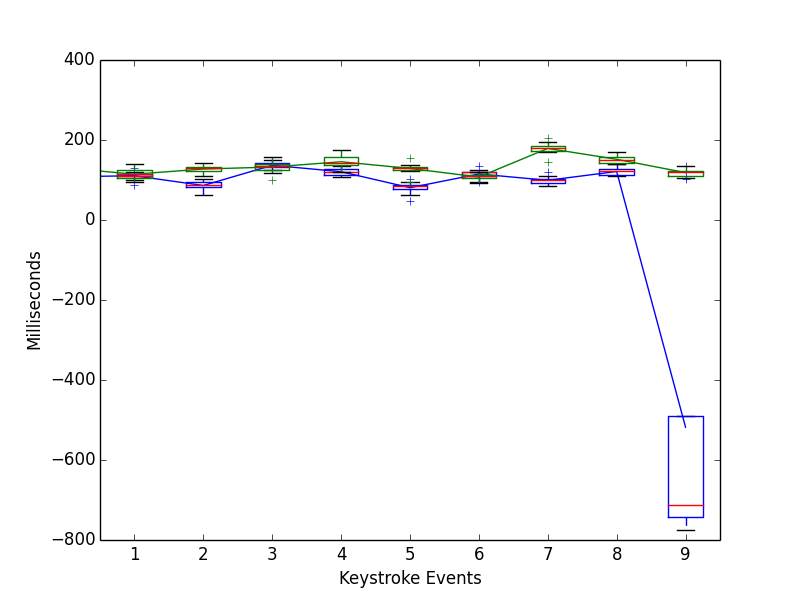
\includegraphics[width=\textwidth]{biedenharn_jordan_dwell_final.png}
    \caption{dwell}
    \label{all_graphs:dwell}
  \end{subfigure}

  \begin{subfigure}[b]{0.3\textwidth}
    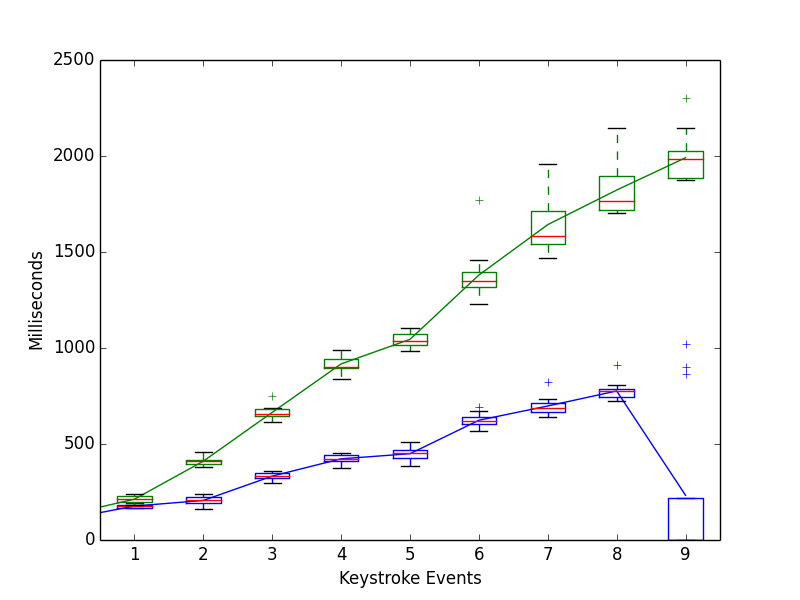
\includegraphics[width=\textwidth]{biedenharn_jordan_up_final.png}
    \caption{up}
    \label{all_graphs:up}
  \end{subfigure}%
  ~ %add desired spacing between images, e. g. ~, \quad, \qquad etc.
    %(or a blank line to force the subfigure onto a new line)
  \begin{subfigure}[b]{0.3\textwidth}
    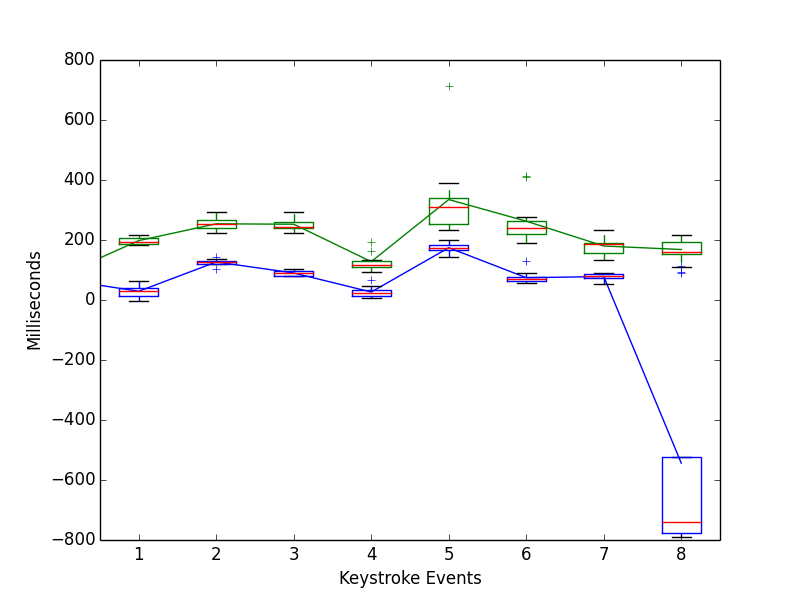
\includegraphics[width=\textwidth]{biedenharn_jordan_up-up_final.png}
    \caption{up-up}
    \label{all_graphs:up-up}
  \end{subfigure}
  ~ %add desired spacing between images, e. g. ~, \quad, \qquad etc.
    %(or a blank line to force the subfigure onto a new line)
  \begin{subfigure}[b]{0.3\textwidth}
    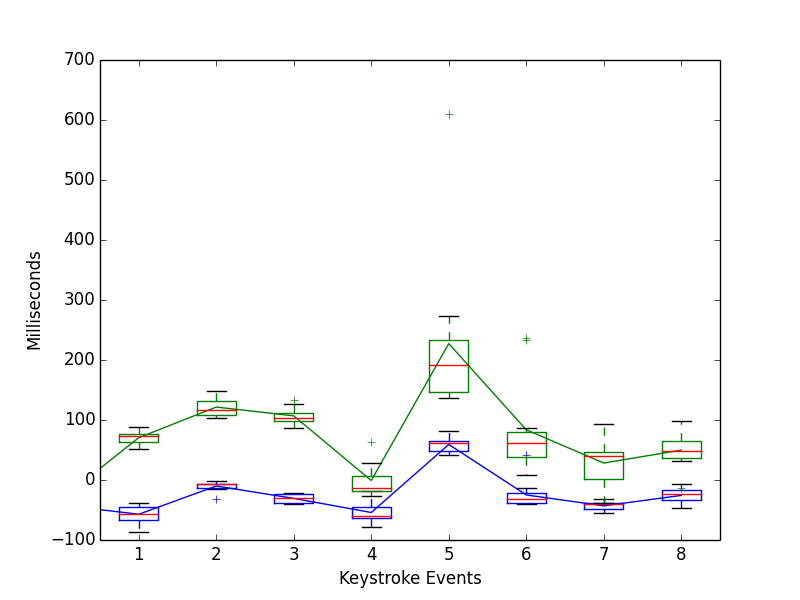
\includegraphics[width=\textwidth]{biedenharn_jordan_flight_final.png}
    \caption{flight}
    \label{all_graphs:flight}
  \end{subfigure}
  \caption{Comparison of the six features. The blue data represents the phrase \textit{biedenharn} typed by somebody familiar with the phrase. The green data represents somebody unfamilar with the phrase.}
  \label{all_graphs}
\end{figure}

\section{Conclusion}
KeystrokeAuth does not intend to be a complete solution to password theft and user authentication. Instead, it is a model client/server website that provides much stronger authentication with minimal inconvenience. We gathered a significant dataset to test against an array of keystroke models and algorithms. The system is very usable with the thresholds we set, but the false negative rate could be even lower with much more data collection and tuning.

Additionally, the implementation is designed to make expansions to the algorithm easier. For example, a weighted mixture of models and algorithms could be used to decide whether a login is successful. Also, the training set could be updated as successful login attempts are made. However, this is risky in that an adversary could potentially skew the training data away from the actual user.

An attempt at a secure, practical, keystroke-based authenticator not been made before this project. We believe that KeystrokeAuth shows that this is a very functional system for password authentication that should be more widely used to protect users.


\begin{thebibliography}{99}
  \bibitem{Killourhy09}
    %comparison of various keystroke timing schemes
   Killourhy, Kevin S., and Roy A. Maxion. 
   ``Comparing anomaly-detection algorithms for keystroke dynamics.''
   \textit{Dependable Systems \& Networks, 2009. DSN'09. IEEE/IFIP International Conference on.}
   IEEE, 2009. 
 
 \bibitem{Cho00}
    %Nearest-neighbor mahalanobis
   Cho, Sungzoon, et al.
   ``Web-based keystroke dynamics identity verification using neural network.'' 
   \textit{Journal of organizational computing and electronic commerce}
   10.4 (2000): 295-307.
  
\end{thebibliography}

\end {document}
